\documentclass[11pt, a4paper]{article}

\usepackage[utf8]{inputenc} % comment when using lualatex
\usepackage[italian]{babel} % lingua e a-capo-sillabato
\usepackage{graphicx}
\usepackage[hidelinks]{hyperref} % link di pagina
\usepackage[bottom]{footmisc} % note appiccicate al fondo della pagina
\usepackage{float} % per posizionamento immagini
\usepackage{amsthm} % per ambienti stile teorema
\usepackage{tabularx} %tabelle
\usepackage[table]{xcolor} %colore caselle
\usepackage{enumitem} %additional commands for lists
\usepackage{fancyhdr}
\usepackage[font=footnotesize,labelfont=bf]{caption} % small caption font-size
\usepackage{afterpage} %fancy does not include page numbers by default

\fancyhf{}% Clear header/footer
\pagestyle{fancy}
\fancyfoot[C]{\thepage} %add page number
\fancyhead[C]{\footnotesize\textit{Documento:} D2 \hfill Sleep Code \hfill \textit{Versione:} 1.0}
\renewcommand{\headrule}{{\color{red!70}\rule{\textwidth}{2pt}}}
\setlength{\headheight}{22pt}

\renewcommand\UrlFont{\color{blue}\rmfamily} % colore link

\theoremstyle{definition} % stile dei newtheorem (non italizzati)
\newtheorem{funcreq}{RF} %% numerazione dei requisiti funzionali
\newtheorem{nonfuncreq}{RNF} %% requisiti non funzionali
\newtheorem{backend}{BE}
\newtheorem{frontend}{FE}




\title{Specifica dei Requisiti}

\author{Raffaele \textsc{Castagna}\\
Alberto \textsc{Rovesti}\\
Zeno \textsc{Saletti}}

\newcommand{\groupNumber}{G17}

% Web address for the project (if any)
% \newcommand{\homepage}{\url{https://www.}}

% data
\date{\today}

\makeatletter{}

\newcommand\blfootnote[1]{%
  \begingroup
  \renewcommand\thefootnote{}\footnote{#1}%
  \addtocounter{footnote}{-1}%
  \endgroup
}

% IL PREAMBOLO FINISCE QUI %%%%%%%%%%%%%%%%%%%%%%%%%%%%%%%%%%%%%%%%%%%%%%%%%%%%



\begin{document}

% La pagina di copertina si trova in un file .tex a parte
% NON MODIFICARE QUESTO COMANDO!!!
\begin{titlepage}
\newcommand{\HRule}{\rule{\linewidth}{0.3mm}} % Defines a new command for horizontal lines, change thickness here
\center % Centre everything on the page

%------------------------------------------------
%	Logo
%------------------------------------------------

\includegraphics[width=0.3\textwidth]{materiale/UniTrento_logo_ITA_colore.png}\\[0.5cm]
%------------------------------------------------
%	Headings
%------------------------------------------------
\textsc{\Large Dipartimento di Ingegneria\\e Scienza dell'Informazione}\\[1.5cm]

{\Huge\textbf{Sleep Code}}\\[0.5cm]
\textsc{\large Progetto per il Corso di Ingegneria del Software}\\
\textsc{\large Anno Accademico 2023-2024}\\[0.5cm]

%------------------------------------------------
%	Title
%------------------------------------------------

\HRule\\[0.4cm]
{\huge\bfseries \@title}\\[0.1cm]
\HRule\\[1cm]

\begin{minipage}{\textwidth}
\begin{flushleft}
\textit{Descrizione:} documento di analisi dei requisiti funzionali, non funzionali, front-end e back-end.
\end{flushleft}
\end{minipage}\\[1.5cm]


\begin{minipage}{0.4\textwidth}
\begin{flushleft}
\large
\textit{Numero documento:} D1
\end{flushleft}
\end{minipage}
\begin{minipage}{0.4\textwidth}
\begin{flushright}
\large
\textit{Versione documento:} 2.4
\end{flushright}
\end{minipage}\\[1.5cm]

%------------------------------------------------
%	Author(s)
%------------------------------------------------
\begin{minipage}{0.4\textwidth}
\begin{flushleft}
\large
\textit{Membri del gruppo:}\\
\@author % Your name
\end{flushleft}
\end{minipage}
~
\begin{minipage}{0.4\textwidth}
\begin{flushright}
\large
\textit{Numero gruppo: }
\groupNumber
\end{flushright}
\end{minipage}

% 	If you don't want a supervisor, uncomment the two lines below and comment the code above
% 	{\large\textit{Author(s)}}\\
% 	\@author % Your name

%------------------------------------------------
%	Date
%------------------------------------------------

\vfill\vfill
\textit{Ultima revisione:}
{\@date}

\end{titlepage}

\tableofcontents\blfootnote{\textbf{Consigli utili per la consultazione del testo:} Se il lettore per file \texttt{.pdf} attualmente in uso lo consente, è possible navigare con più semplicità e velocità all'interno di questo documento cliccando sugli elementi dell'indice.}

\afterpage{\cfoot{\thepage}}
\newpage
\section*{Scopo del documento}
Il presente documento riporta la specifica dei requisiti di sistema
del progetto Sleep Code. Viene in particolare estesa la descrizione
in linguaggio naturale, impiegato nel documento di Analisi dei Requisiti
(D1), attraverso strumenti di modellazione più formali—diagrammi
realizzati secondo gli standard indicati da \textit{Unified Modeling Language}
(UML) per quanto riguarda i requisiti funzionali; tabelle strutturate
per i requisiti non funzionali.

In ultima analisi, contemplando i suddetti requisiti, viene presentato il
design del sistema ricorrendo ai diagrammi di contesto e dei componenti.


\newpage
\section{Requisiti funzionali}
In questa sezione vengono descritti i requisiti funzionali (RF) del
progetto, evidenziando la partecipazione degli attori esterni, ovvero
l'utente finale e i servizi esterni di back-end (BE) a supporto del progetto. A tal
proposito, vengono utilizzati Use Case Diagrams (UCD) e Swimlane Diagrams (SD),
disegnati secondo gli standard UML, ed eventualmente arricchiti da
descrizioni in linguaggio naturale\footnote{Gli use cases più semplici
presenti nei diagrammi non vengono descritti in altri modi, in quanto ritenuti
autoesplicativi.}.

\subsection{Accesso e autenticazione}\label{accessoeautenticazione}
La Figura \ref{access} mostra gli use cases che rappresentano i seguenti
requisiti funzionali: \textbf{RF 1} - Registrazione,
\textbf{RF 2} - Login, \textbf{RF 3} - Autenticazione Google, \textbf{RF 4} - Recupero
password.

\begin{figure}[H]
\centering
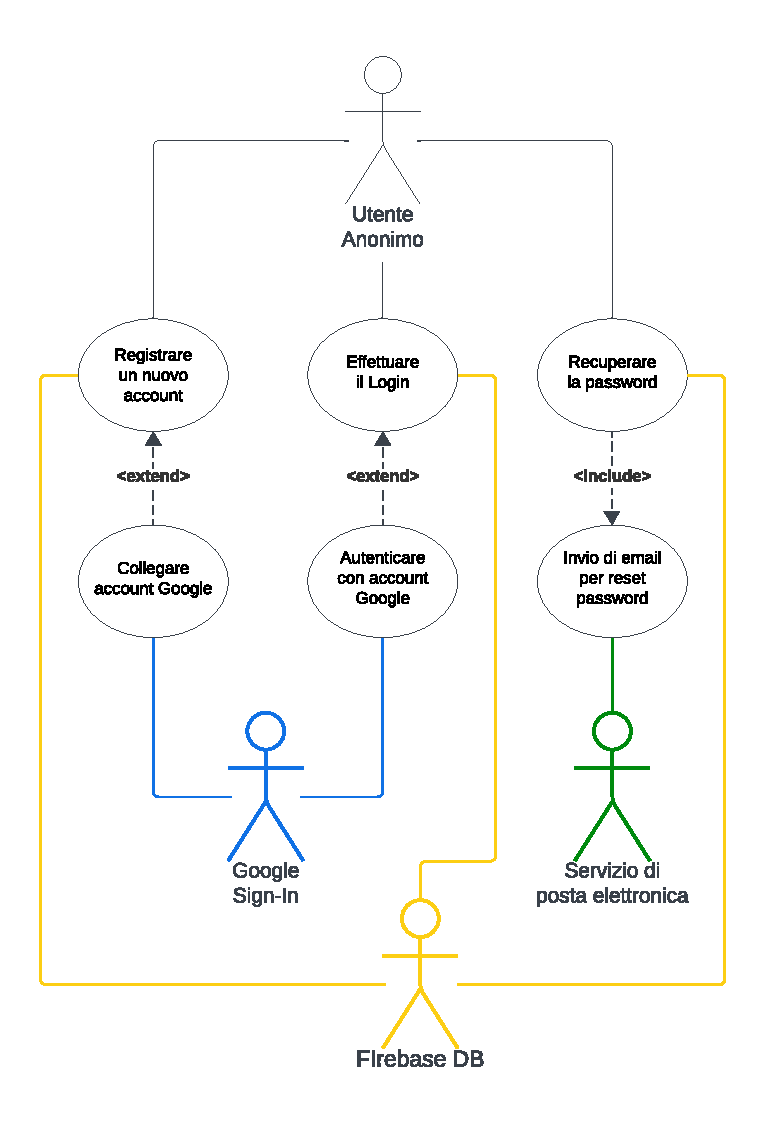
\includegraphics[scale=0.63]{materiale/ucdiagrams/ucaccesso.pdf}
\caption{UCD relativo ai RF inerenti all'accesso alla piattaforma}
\label{access}
\end{figure}

\subsection*{Descrizione Use Case \textit{Registrare un nuovo account}}
\begin{description}
    \item[Titolo:] Registrazione account
    
    \item[Riassunto:] Questo Use Case descrive come l'utente anonimo deve
    effettuare la registrazione sulla piattaforma.

    \item[Descrizione:]
    \begin{enumerate}
        \item[]
        \item L'utente anonimo accede alla pagina dedicata, raggiungibile da quella di login, e sceglie la modalità di registrazione con il sistema di credenziali interno.\texttt{[extension 1]}
        \item La registrazione con sistema di credenziali interno prevede l'inserimento di un username, un'email e una password conforme. \verb|[exception 1]|
        \item La password deve essere confermata reinserendola in un secondo campo.\verb|[exception 2]|
        \item I dati vengono raccolti e il relativo account viene registrato dal servizio di database.\texttt{[exception 3]}
        \item L'utente riceve una conferma circa l'esito dell'operazione di registrazione.
    \end{enumerate}
    
    \item[Exceptions:]
    \begin{itemize}
        \item[]
        \item \texttt{[exception 1]} Se la password non è conforme, la registrazione non può proseguire e l'utente viene avvisato.
        \item \texttt{[exception 2]} Se i campi di inserimento e di conferma della password contengono stringhe che non coincidono, la registrazione non può proseguire e l'utente viene avvisato.
        \item \texttt{[exception 3]} Se l'email inserita dall'utente risulta essere già impiegata in un altro account, la registrazione non può proseguire e l'utente viene avvisato.
    \end{itemize}

    \item[Extensions:]
    \begin{itemize}
        \item[]
        \item \texttt{[extension 1]} In alternativa, l'utente può scegliere di registrarsi alla piattaforma collegando un account Google in suo possesso, secondo quanto indicato dal servizio di registrazione e autenticazione Google.
        In questo caso, oltre a scegliere l'email come previsto dal servizio di Google, l'utente specifica l'username.
    \end{itemize}
\end{description}

\newpage
\subsection*{Descrizione Use Case \textit{Effettuare il login}}
\begin{description}
    \item[Titolo:] Login
    
    \item[Riassunto:] Questo Use Case descrive come l'utente anonimo e registrato deve
    effettuare il login sulla piattaforma.

    \item[Descrizione:]
    \begin{enumerate}
        \item[]
        \item L'utente anonimo accede alla pagina di login.\texttt{[extension 1]}
        \item L'utente che si autentica con credenziali interne inserisce indirizzo email e password, che saranno verificati grazie al servizio di database.\texttt{[exception 1]}
        \item L'utente riceve la conferma di login.
    \end{enumerate}
    
    \item[Exceptions:]
    \begin{itemize}
        \item[]
        \item \verb|[exception 1]| Se le credenziali fornite non sono valide, il login non può essere eseguito e l'utente viene avvisato.
        È comunque possibile ritentare il login, senza alcun limite nel numero di tentativi.
    \end{itemize}

    \item[Extensions:]
    \begin{itemize}
        \item[]
        \item \texttt{[extension 1]} Qualora l'utente disponga di un account Google collegato alla piattaforma, è possibile effettuare il login
        mediante autenticazione Google e seguendo le indicazioni fornite dal suo servizio.
    \end{itemize}
\end{description}

\subsection*{Descrizione Use Case \textit{Recuperare la password}}
\begin{description}
    \item[Titolo:] Recupero password
    
    \item[Riassunto:] Questo Use Case descrive come l'utente anonimo e
    registrato alla piattaforma, facendo affidamento al sistema di credenziali
    interno, può recuperare il proprio account qualora la password venisse dimenticata.

    \item[Descrizione:]
    \begin{enumerate}
        \item[]
        \item L'utente accede alla pagina di recupero, attraverso quella di login.
        \item La pagina indica all'utente di inserire l'email di recupero, ovvero quella attualmente associata all'account. \verb|[exception 1]|
        \item Il sistema richiede al servizio di posta elettronica l'invio di un link di recupero mediante un messaggio email, specificando l'indirizzo fornito dall'utente e il contenuto del messaggio.
        \item Il link guida l'utente dal messaggio alla pagina del sistema dedicata alla creazione di una nuova password.
        \item L'utente inserisce una nuova password conforme e la conferma, inserendola nuovamente. \verb|[exception 2]|
        \item Il servizio di database provvede all'aggiornamento della password.
    \end{enumerate}
    
    \item[Exceptions:]
    \begin{itemize}
        \item[]
        \item \verb|[exception 1]| Se l'email inserita non è associata ad alcun account registrato, il recupero non può proseguire e l'utente viene avvisato.
        \item \verb|[exception 2]| Se la password non è conforme, oppure se i campi di inserimento e conferma della password contengono stringhe che non coincidono, la registrazione non può proseguire e l'utente viene avvisato.
    \end{itemize}
    
    %\item[Extensions:]
\end{description}


\newpage
\subsection{Consultazione e gestione dei problemi}\label{consultazione}
In Figura \ref{catalogueprobs} sono mostrati gli use cases che illustrano
le funzionalità che interessano l'utente (anonimo, autenticato e amministratore)
nell'ambito della constultazione del catalogo e del contenuto
dei problemi. In particolar modo, sono state isolate nel diagramma le funzionalità
fruibili nella pagina del catalogo e nella pagina di consultazione
del singolo problema dell'area di esercitazione (\textbf{FE 3} e \textbf{FE 4}
nel documento D1).

I requisiti descritti sono: \textbf{RF 5} - Consultazione del catalogo,
\textbf{RF 6} - Consultazione di un problema, \textbf{RF 10} - Metadati aggiuntivi,
\textbf{RF 12.2} - Visualizzare i Progressi, \textbf{RF 16} - Aggiungere un problema,
\textbf{RF 17} - Modificare un problema, \textbf{RF 18} - Eliminare un problema.
Questi ultimi tre, relativi all'utente amministratore, sono riassunti nello use case
\textit{Modificare il catalogo dei problemi}, che include le tre azioni opzionali (da
cui le clausole \texttt{extend} nel diagramma).


\begin{figure}[H]
\centering
\hspace*{-1.7cm}
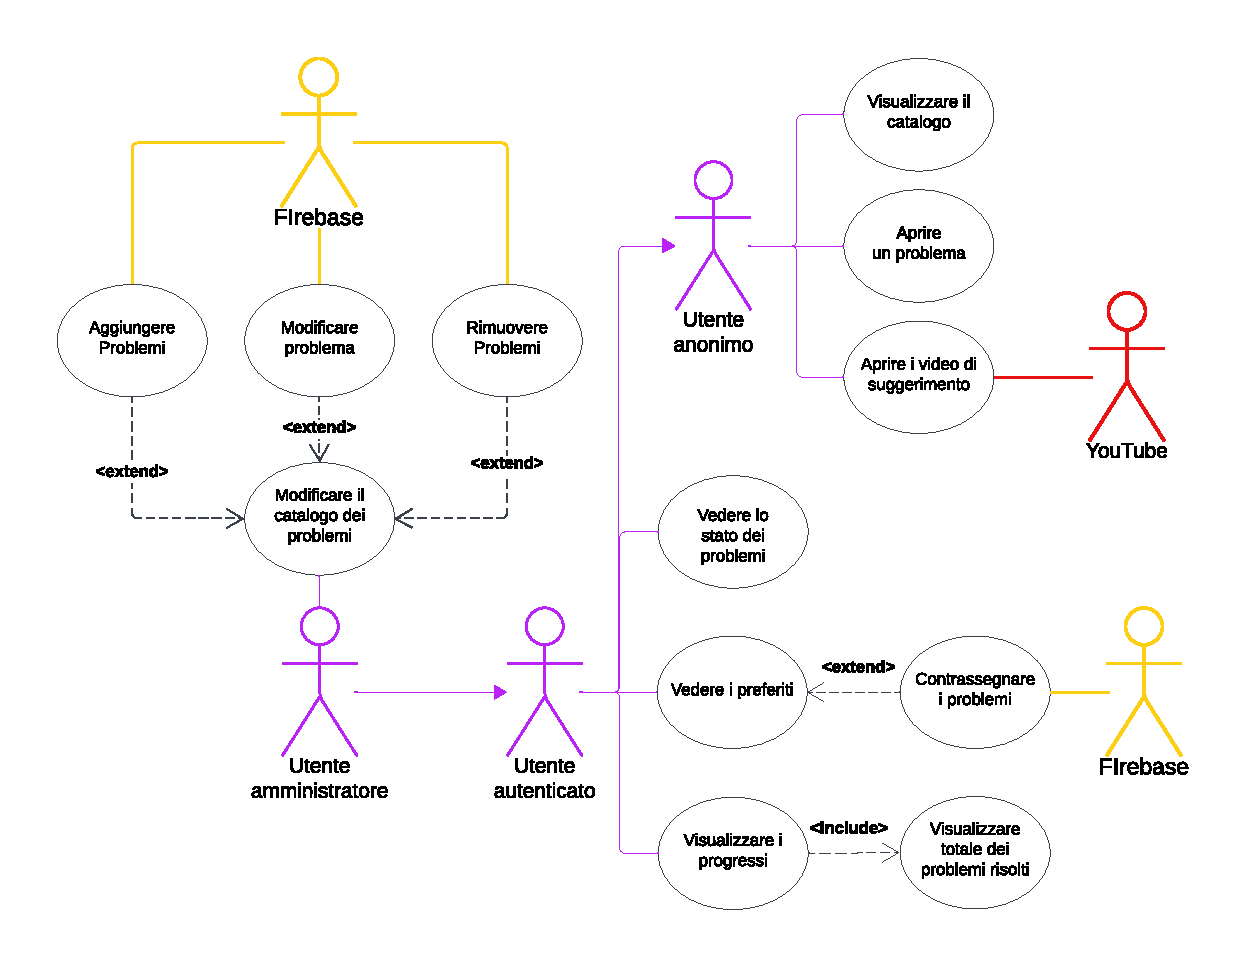
\includegraphics[scale=0.76]{materiale/ucdiagrams/ucproblemi.pdf}
\caption{UCD relativo alla consultazione dei problemi, modifica del catalogo e visualizzazione progressi}
\label{catalogueprobs}
\end{figure}

\newpage
\subsection*{Descrizione Use Case \textit{Aggiungere problemi}}
\begin{description}
    \item[Titolo:] Aggiungere un problema
    
    \item[Riassunto:] Questo Use Case descrive come l'utente amministratore
    deve aggiungere nuovi problemi al catalogo.

    \item[Descrizione:]
    \begin{enumerate}
        \item[]
        \item L'utente amministratore accede alla pagina del catalogo e sceglie di aggiungere un nuovo problema.
        \item L'utente compila i campi necessari alla creazione di un nuovo problema: i dati relativi alla struttura, quali titolo, descrizione e almeno due esempi di input e output atteso; dati descrittivi, ovvero nome, selezione della difficoltà (bassa, intermedia, alta), categoria e link di YouTube al video-suggerimento.
        \item L'utente inserisce almeno 3 test cases; ogni test case consiste in un dato in input e il rispettivo output corretto.
        \item L'utente conferma la creazione del problema, che viene quindi aggiunto al catalogo; alternativamente, l'utente può scegliere di annullare la creazione del nuovo problema, previo avviso e conferma da parte del sistema.\texttt{[exception 1]}\texttt{[exception 2]}
    \end{enumerate}
    
    \item[Exceptions:]
    \begin{itemize}
        \item[]
        \item \texttt{[exception 1]} Se tra i dati strutturali e descrittivi del problema è presente almeno un campo non compilato, l'aggiunta del problema al catalogo non viene eseguita e l'utente viene avvisato.
        \item \texttt{[exception 2]} Se il numero di test cases forniti è minore di 3, il problema non può essere aggiunto e l'utente viene notificato.
    \end{itemize}
\end{description}

\subsubsection*{Descrizione Use Case \textit{Modificare problemi}}
\begin{description}
    \item[Titolo:] Modificare un problema
    
    \item[Riassunto:] Questo Use Case descrive come l'utente amministratore
    deve modificare i problemi.

    \item[Descrizione:]
    \begin{enumerate}
        \item[]
        \item L'utente amministratore accede alla pagina del catalogo e seleziona un problema da modificare.
        \item L'utente modifica i campi strutturali (titolo, descrizione, esempi di input e output) e descrittivi (nome, difficoltà, categoria e link al video-suggerimento) del problema.
        \item L'utente modifica i test cases, aggiungendone eventualmente più di 3.
        \item L'utente conferma la modifica del problema, che verrà poi aggiornato nel catalogo, oppure conferma di annullare la modifica.\texttt{[exception 1]} \texttt{[exception 2]}
    \end{enumerate}
    
    \item[Exceptions:]
    \begin{itemize}
        \item[]
        \item \texttt{[exception 1]} Se tra i dati strutturali e descrittivi del problema è presente almeno un campo non compilato, la modifica del problema non viene eseguita e l'utente viene avvisato.
        \item \texttt{[exception 2]} Se il numero di test cases forniti è minore di 3, il problema non può essere modificato e l'utente viene notificato.
    \end{itemize}
\end{description}

\newpage
\subsection{Esercitazione}
La Figura \ref{esercitaz} raggruppa use cases associati ai requisiti funzionali
che costituiscono l'area di esercitazione dello specifico problema. Pertanto,
i requisiti rappresentati qui sono i seguenti: \textbf{RF 7} - Effettuare l'esercitazione,
\textbf{RF 8} - Verifica della correttezza dell'algoritmo, \textbf{RF 9} - Cronometro,
\textbf{RF 11} - Codice, \textbf{RF 12.1} - Registrazione dei Progressi. Dal punto di
vista del frontend, il diagramma raccoglie gran parte delle funzionalità utilizzabili
interagendo con gli strumenti dell'area di esercitazione visibili in \textbf{FE 4}.

\begin{figure}[H]
\centering
\hspace*{-2cm}
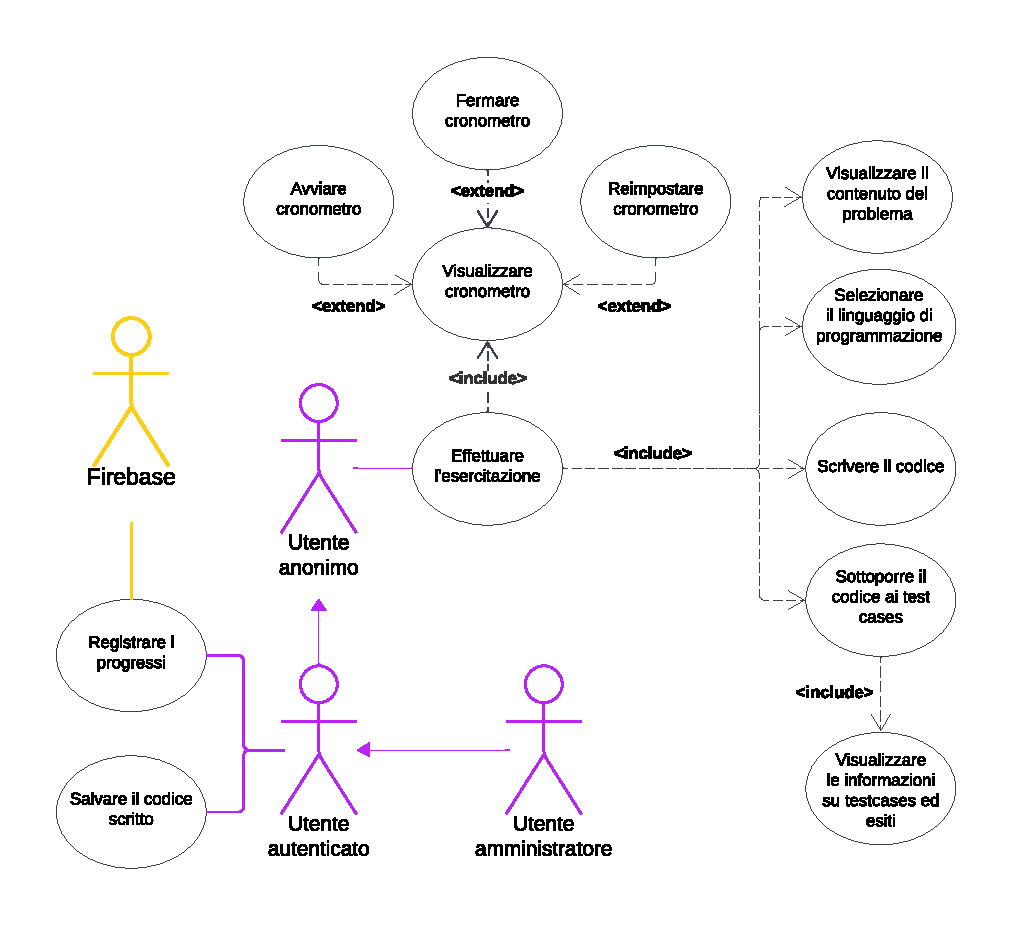
\includegraphics[scale = 0.95]{materiale/ucdiagrams/ucesercitazione.pdf}
\caption{UCD con riferimenti ai requisiti relativi ai tools di esercitazione}
\label{esercitaz}
\end{figure}

\newpage
\subsection*{Descrizione dell'esercitazione}
La complessità delle operazioni relative all'esercitazione è
catturata dalla Figura \ref{acexercise}.
Dal momento che l'utente può decidere di uscire dall'area di esercitazione
a propria discrezione, il processo descritto nel diagramma
può essere interrotto in qualsiasi momento, prima che tutti i
testcases vengano risolti.
La corsia \textit{Firebase} descrive le
attività previste dallo use case \textit{Registrare i progressi}
(Figura \ref{esercitaz}), tenendo ovviamente in conto l'utente
autenticato del quale aggiornare i progressi.
Si assume che l'attività \textit{Visualizza cronometro} includa
implicitamente le funzionalità descritte dal relativo use case.

\begin{figure}[H]
\centering
%\hspace*{-0.4cm}
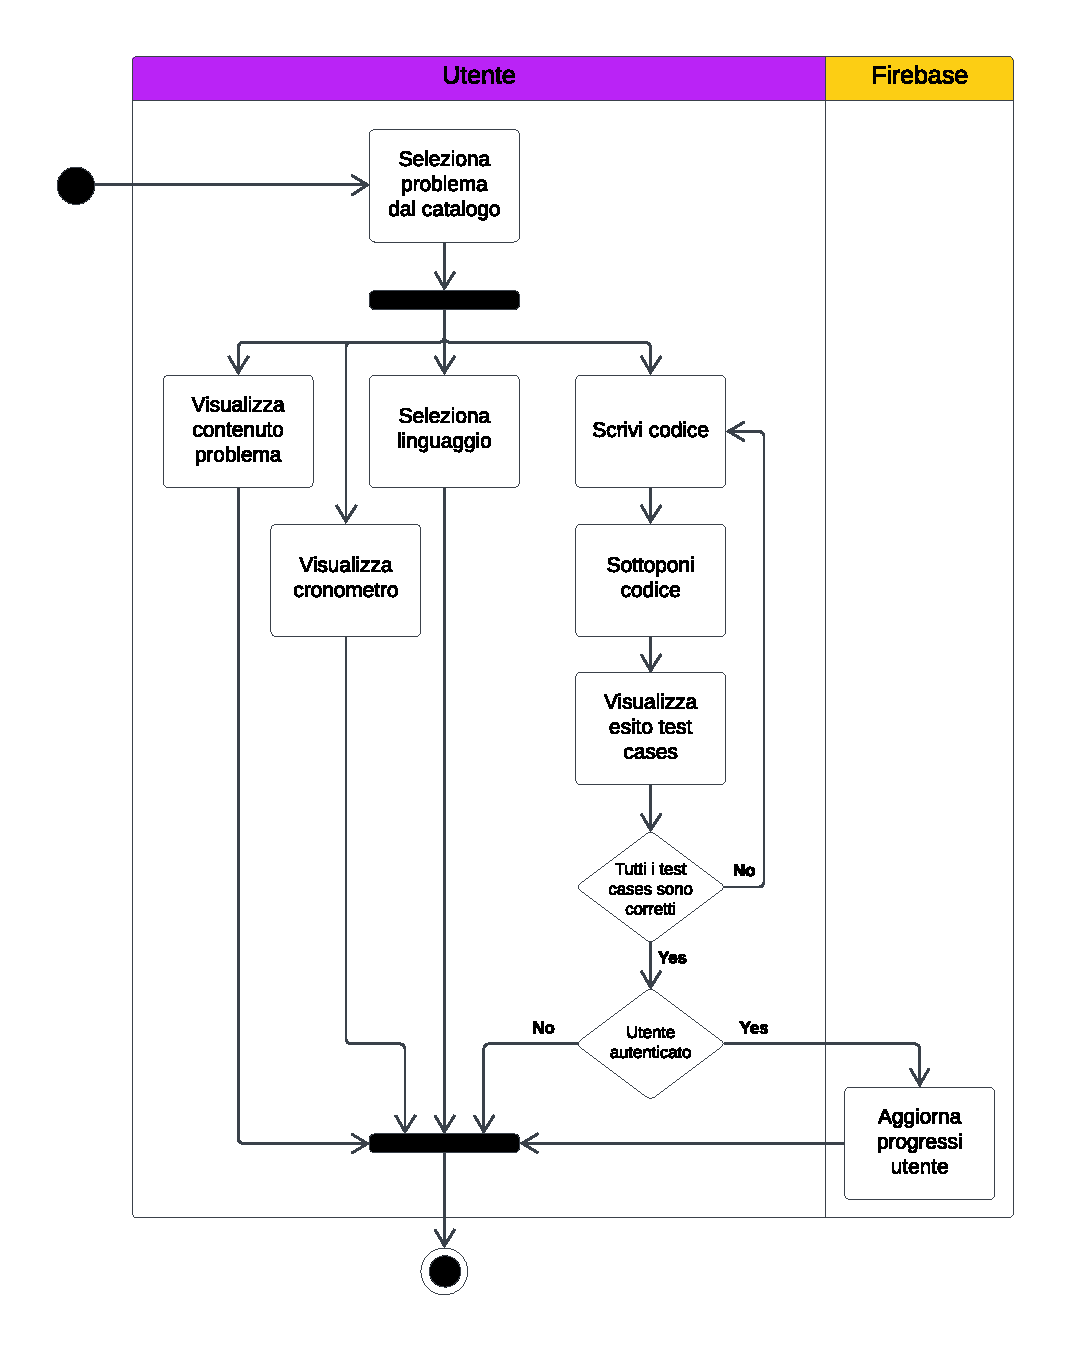
\includegraphics[scale=0.65]{materiale/ucdiagrams/swimlaneesercitazione.pdf}
\caption{SD, arricchito da elementi di Activity Diagram,
per gli use case \textit{Effetuare l'esercitazione}, gli use case correlati
e \textit{Registrare i progressi}}
\label{acexercise}
\end{figure}


\newpage
\subsection{Gestione dell'account}
In Figura \ref{accountfig} sono riassunti gli use cases che descrivono
le operazioni possibili per gli utenti autenticati dotati di account. Come già accennato
nel documento D1, \textit{Aggiornare l'indirizzo email dell'account} e
\textit{Aggiornare la password dell'account} sono possibili solo a utenti
autenticati con sistema di credenziali interno. Questo fatto è appunto
sottolineato dalla presenza dell'attore \textit{Firebase}. Si fa riferimento
ai seguenti requisiti funzionali:
\textbf{RF 13} - Aggiornamento password, \textbf{RF 14} - Logout,
\textbf{RF 15} - Eliminazione account.

\begin{figure}[H]
\centering
%\hspace*{-1.8cm}
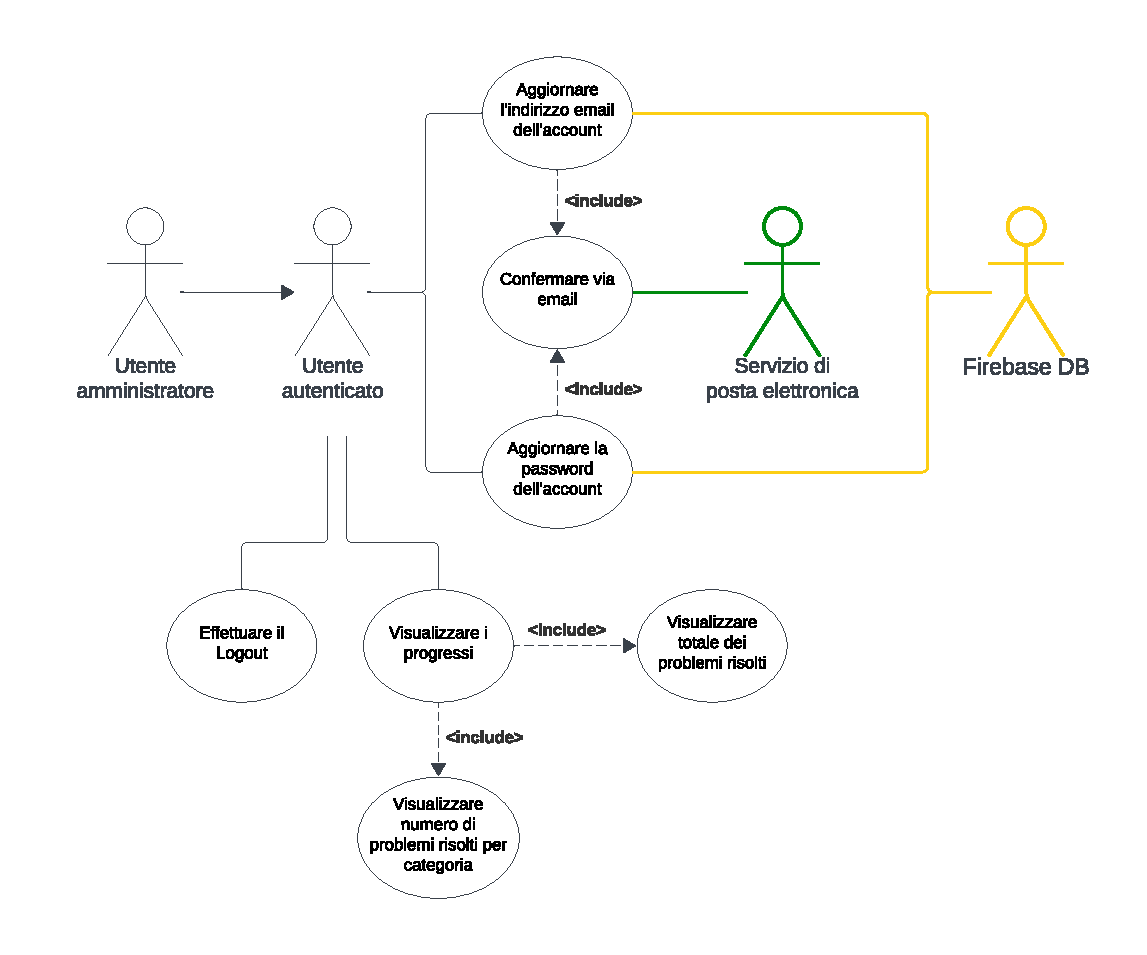
\includegraphics[scale = 0.88]{materiale/ucdiagrams/ucaccount.pdf}
\caption{UCD relativo alle funzionalità dell'account}
\label{accountfig}
\end{figure}



\newpage
\subsection*{Descrizione Use Case \textit{Aggiornare la password dell'account}}
La Figura \ref{slpassword} fa riferimento allo Use Case relativo all'aggiornamento
della password dell'account di un utente registrato con credenziali di sistema e autenticato.
Durante il processo di aggiornamento, l'utente ha la facoltà di interrompere
la procedura qualora non intenda più modificare la password, purché ciò avvenga
prima della conferma.

\begin{figure}[H]
\centering
\hspace*{-0.7cm}
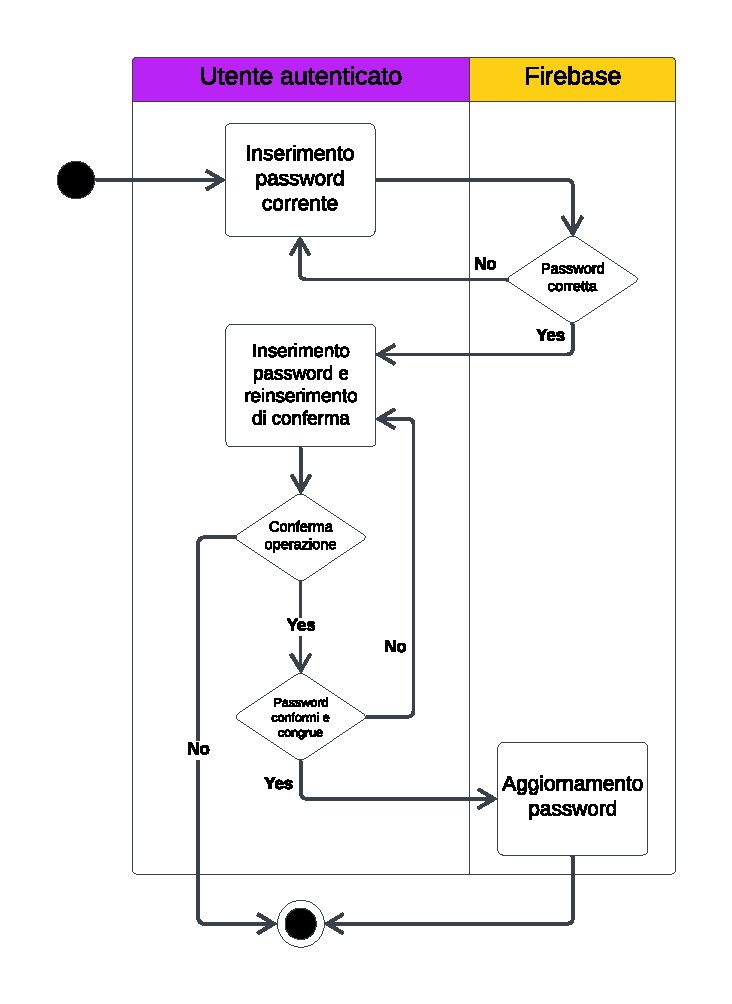
\includegraphics[scale = 1]{materiale/ucdiagrams/swimlanepassword.pdf}
\caption{SD dello scenario di aggiornamento della password}
\label{slpassword}
\end{figure}

\newpage
\subsection*{Descrizione Use Case \textit{Eliminazione account}}
Lo Swimlane Diagram rappresentato in Figura \ref{deleteaccount} mostra
i dettagli dello Use Case \textit{Eliminazione account}. In seguito
all'eliminazione, l'utente interessato ritorna al livello di accesso
anonimo.

\begin{figure}[H]
\centering
%\hspace*{-0.7cm}
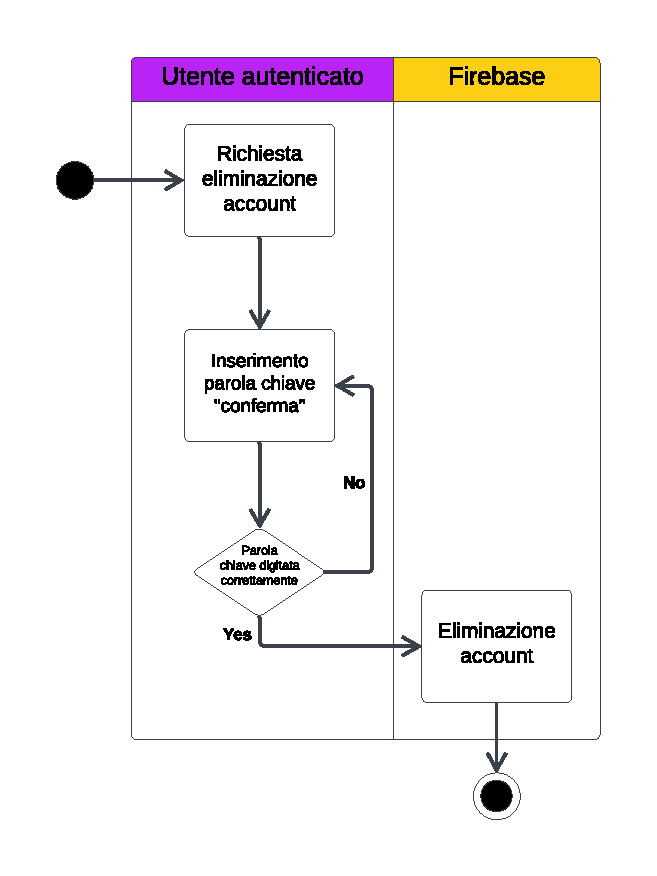
\includegraphics[scale = 1]{materiale/ucdiagrams/swimlaneeliminaaccount.pdf}
\caption{SD per lo Use Case \textit{Eliminazione account}}
\label{deleteaccount}
\end{figure}

\newpage
\section{Requisiti non funzionali}
Di seguito sono riportati i requisiti non funzionali (RNF)
del sistema, all'interno di tabelle strutturate. Per ogni requisito vengono
specificate una o più proprietà con una descrizione più esplicita,
oltre ad un indice di misura utile alla valutazione oggettiva
e quantitativa di tali requisiti.

\subsection{Caratteristiche di sistema}

\begin{nonfuncreq}
\textbf{Scalabilità }
\begin{center}
    \footnotesize
    \begin{tabularx}{\textwidth}{|X||X||X|}
        \hline
        \cellcolor{red!70}Proprietà & \cellcolor{red!70}Descrizione & \cellcolor{red!70}Misura\\
        \hline
        Elaborazione con un numero crescente di utenti & Capacità del sistema di gestire un numero crescente di utenti in simultanea. & Viene garantito l'accesso in simultanea di almeno 300 utenti nel primo anno dal lancio.\\
        \hline
        Memorizzazione dei dati degli utenti & Capacità del sistema di gestire i dati generati da un numero crescente di utenti utilizzatori. & Capacità sufficiente per almeno 400 utenti.\\
        \hline
        Eterogeneità dei linguaggi di programmazione & Capacità di supportare un numero crescente di linguaggi di programmazione, utili alla scrittura degli algoritmi risolutivi. & Al lancio della piattaforma, viene supportato JavaScript. Il sistema potrà gestire algoritmi scritti in almeno 5 linguaggi differenti.\\
        \hline
    \end{tabularx}
\end{center}
\end{nonfuncreq}

\begin{nonfuncreq}
    \textbf{Compatibilità }
    \begin{center}
        \footnotesize
        \begin{tabularx}{\textwidth}{|X||X||X|}
            \hline
            \cellcolor{red!70}Proprietà & \cellcolor{red!70}Descrizione & \cellcolor{red!70}Misura\\
            \hline
            Compatibilità client & La piattaforma del servizio deve essere compatibile con e accessibile attraverso le versioni più recenti dei principali browser in commercio. &
            \begin{itemize}
                \item Chrome

                117.0.5938.150
                \item Firefox

                18.0.1
                \item Edge:

                17.0.2045.60
            \end{itemize}La compatibilità deve valere anche per le rispettive versioni superiori.\\
            \hline
        \end{tabularx}
    \end{center}
\end{nonfuncreq}

\begin{nonfuncreq}
    \textbf{Usabilità }
    \begin{center}
        \footnotesize
        \begin{tabularx}{\textwidth}{|X||X||X|}
            \hline
            \cellcolor{red!70}Proprietà & \cellcolor{red!70}Descrizione & \cellcolor{red!70}Misura\\
            \hline
            Usabilità & Intuitività e facilità nell'apprendimento, accesso e impiego delle funzionalità fornite dal servizio. & Il nuovo utente deve poter conoscere e utilizzare il 90\% (rapporto tra RF scoperti e RF totali) delle funzionalità disponibili al proprio livello di accesso in meno di 30 minuti.\\
            \hline
        \end{tabularx}
    \end{center}
\end{nonfuncreq}

\begin{nonfuncreq}
    \textbf{Aspetto }
    \begin{center}
        \footnotesize
        \begin{tabularx}{\textwidth}{|X||X||X|}
            \hline
            \cellcolor{red!70}Proprietà & \cellcolor{red!70}Descrizione & \cellcolor{red!70}Misura\\
            \hline
            Colore & Gamma cromatica dell'interfaccia e distribuzione del colore. La scelta ricade su colori, tinte (aggiunta di bianco) e sfumature (aggiunta di nero) che mirano a limitare l'affaticamento della vista. & Colori caldi; colori freddi presenti in sfumature scure; colori freddi accesi presenti al più in aree ristrette (pulsanti e icone).\\
            \hline
            Contrasto & Accostamento dei colori all'interno dell'interfaccia utente. Mira alla leggibilità e alla limitazione dell'affaticamento della vista. & Regola dei complementari; cerchio di Itten.\\
            \hline
            Segnalazioni grafiche di attesa & Indicazioni visive che notificano all'utente lo stato di caricamento delle pagine, in particolare durante le transizioni client-server. & Impiego di skeleton screens per le transizioni, popup per le operazioni di autenticazione.\\
            \hline
        \end{tabularx}
    \end{center}
\end{nonfuncreq}

\begin{nonfuncreq}
    \textbf{Lingua }
    \begin{center}
        \footnotesize
        \begin{tabularx}{\textwidth}{|X||X||X|}
            \hline
            \cellcolor{red!70}Proprietà & \cellcolor{red!70}Descrizione & \cellcolor{red!70}Misura\\
            \hline
            Lingua di sistema           & Lingua presente nell'interfaccia e nelle risorse fornite dal servizio. & Percentuale di testo scritto in una data lingua. L'interfaccia generale della piattaforma contiene testo in italiano (100\%); al lancio del servizio, i testi dei problemi saranno scritti in italiano (100\%); le risorse multimediali (video-suggerimento) devono essere in italiano oppure in inglese.\\
            \hline
        \end{tabularx}
    \end{center}
\end{nonfuncreq}

\begin{nonfuncreq}
    \textbf{Prestazioni }
    \begin{center}
        \footnotesize
        \begin{tabularx}{\textwidth}{|X||X||X|}
            \hline
            \cellcolor{red!70}Proprietà & \cellcolor{red!70}Descrizione & \cellcolor{red!70}Misura\\
            \hline
            Caricamento all'accesso & Tempo massimo richiesto per caricare le pagine rilevanti dopo la ricerca in browser. & Il caricamento delle pagine di login e home (per quest'ultima si considera l'intervallo di tempo che comincia dopo la richiesta di autenticazione) non deve eccedere i 2 secondi.\\
            \hline
            Transizioni & Tempo massimo richiesto per effettuare una transizione da una pagina all'altra.  & Una transizione non deve richiedere più di 2 secondi.\\
            \hline
        \end{tabularx}
    \end{center}
\end{nonfuncreq}

\subsection{Affidabilità}

\begin{nonfuncreq}
    \textbf{Downtime }
    \begin{center}
        \footnotesize
        \begin{tabularx}{\textwidth}{|X||X||X|}
            \hline
            \cellcolor{red!70}Proprietà & \cellcolor{red!70}Descrizione & \cellcolor{red!70}Misura\\
            \hline
            Downtime & Tempo medio massimo in cui il servizio non è raggiungibile; principalmente per motivi di manutenzione e aggiornamento. & 2,7\% (240 ore) nel primo anno 0,85\% (72 ore) dopo il primo anno dal lancio.\\
            \hline
        \end{tabularx}
    \end{center}
\end{nonfuncreq}

\begin{nonfuncreq}
    \textbf{Disponibilità }
    \begin{center}
        \footnotesize
        \begin{tabularx}{\textwidth}{|X||X||X|}
            \hline
            \cellcolor{red!70}Proprietà & \cellcolor{red!70}Descrizione & \cellcolor{red!70}Misura\\
            \hline
            Disponibilità & Probabilità che il sito non si guasti entro un intervallo di tempo trascorso dopo l'entrata in servizio. & Probabilità di resistere ai guasti al 98\% entro le prime 8.000 ore.\\
            \hline
        \end{tabularx}
    \end{center}
\end{nonfuncreq}

\subsection{Privacy e sicurezza}

\begin{nonfuncreq}
    \textbf{Privacy e trattamento dei dati }
    \begin{center}
        \footnotesize
        \begin{tabularx}{\textwidth}{|X||X||X|}
            \hline
            \cellcolor{red!70}Proprietà & \cellcolor{red!70}Descrizione & \cellcolor{red!70}Misura\\
            \hline
            Normativa & Conformità con le vigenti norme relative al trattamento e alla protezione dei dati (GDPR). In particolare, i dati personali dell'utente registrato (nome, email e password) non devono essere divulgati in alcun modo e, qualora lo ritenga opportuno, l'utente ha il diritto di richiedere l'eliminazione delle proprie informazioni dal servizio al fine di interrompere il trattamento. & Conformità del servizio e funzionalità a supporto dell'utente (eliminazione account—\textbf{RF 15}—memorizzazione del codice scritto da utenti autenticati solo da parte del client).\\
            \hline
        \end{tabularx}
    \end{center}
\end{nonfuncreq}

\begin{nonfuncreq}
    \textbf{Connessione sicura }
    \begin{center}
        \footnotesize
        \begin{tabularx}{\textwidth}{|X||X||X|}
            \hline
            \cellcolor{red!70}Proprietà & \cellcolor{red!70}Descrizione & \cellcolor{red!70}Misura\\
            \hline
            Connessione sicura & Impiego di protocolli di comunicazione che garantiscono la confidenzialità e riservatezza delle informazioni scambiate tra client e server. & Utilizzo del protocollo \texttt{https}.\\
            \hline
        \end{tabularx}
    \end{center}
\end{nonfuncreq}

\newpage
\begin{nonfuncreq}
    \textbf{Password strength }
    \begin{center}
        \footnotesize
        \begin{tabularx}{\textwidth}{|X||X||X|}
            \hline
            \cellcolor{red!70}Proprietà & \cellcolor{red!70}Descrizione & \cellcolor{red!70}Misura\\
            \hline
            Password sicura & Quantità e varietà di caratteri necessari per comporre una password forte e sicura. & Una password conforme rispetta:
            \begin{itemize}[leftmargin = *]
                \item Numero di caratteri: compreso tra 8 e 64
                \item Maiuscola-minuscola: almeno una lettera maiuscola e una minuscola
                \item Cifra decimale: almeno una cifra decimale
                \item Carattere speciale: almeno un carattere tra  ! ? \# \$ \% \& @ * + - / $\backslash$ = \_ . , ; : ( ) [ ] \{ \}.
            \end{itemize}\\
            \hline
        \end{tabularx}
    \end{center}
\end{nonfuncreq}





\newpage
\section{Analisi del contesto}
% riguarda il backend e i componenti esterni al sistema: tutto il codice che utilizzate ma che non avete scritto voi
% flusso di informazioni tra il nostro sistema e quelli esterni
In questa sezione viene descritto il contesto di funzionamento del sistema
Sleep Code e come esso interagisce con gli attori esterni. Si
ricorre ad una descrizione testuale riassunta in una rappresentazione
grafica mediante un Diagramma di Contesto riportato in
Figura \ref{contextdiagram}, nel quale sono specificati, ad alto livello,
i flussi di informazioni essenziali al funzionamento del sistema.

\subsection{Utenti e sistemi esterni} % chi interagisce, chi usa e chi supporta (sia software che umano)
Sono elencati di seguito gli attori esterni che compongono il contesto
del sistema in sviluppo. Essi fanno riferimento ad alcuni dei requisiti
funzionali definiti nel documento D1 e nei quali si evince la presenza
attiva degli attori, come già mostrato negli UCDs.

\subsubsection{Utente}
L'utente rappresenta l'attore che usufruisce delle funzionalità del servizio
—viene descritto nei requisiti dal \textbf{RF 1} al \textbf{RF 9} per quanto
concerne il livello anonimo e quelli superiori; dal \textbf{RF 10} al
\textbf{RF 15} in relazione ai livelli autenticato e amministratore; \textbf{RF 16},
\textbf{RF 17} e \textbf{RF 18} per quanto riguarda il livello amministratore.

\subsubsection{Firebase}
Il servizio di database impiegato per gestire le credenziali e il profilo
degli utenti registrati alla piattaforma—i requisiti coinvolti sono: \textbf{RF 1},
\textbf{RF 2}, \textbf{RF 3}, \textbf{RF 4}, \textbf{RF 10}, \textbf{RF 12.1},
\textbf{RF 13}, \textbf{RF 15}—e per gestire il catalogo dei problemi—\textbf{RF 5}, \textbf{RF 6},
\textbf{RF 16}, \textbf{RF 17}, \textbf{RF 18}.

\subsubsection{Google Sign-In}
Il servizio di autenticazione alternativo al sistema di credenziali interno
—\textbf{RF 3}.

\subsubsection{YouTube}
Il servizio di contenuti multimediali che fornisce e visualizza i video
che integrano i problemi del catalogo, mettendo a disposizione dell'utente
un suggerimento per lo svolgimento dell'esercizio—\textbf{RF 5.1}.

\subsubsection{Servizio di posta elettronica}
Sistema di notifica sul quale il progetto si poggia per creare un
meccanismo di recupero della password dell'account—\textbf{RF 4}.

\newpage
\subsection{Diagramma di contesto} % frecce = dati che si scambiano. Utente --atuenticaz--> sistema (è l'utente che fornisce i dati al sistema; la freccia indica il verso del flusso)
La Figura \ref{contextdiagram} mostra il diagramma di contesto per il
servizio Sleep Code. Seguono alcune descrizioni più dettagliate
che chiariscono il significato, per lo più ad alto livello, delle
informazioni scambiate tra il sistema e gli attori esterni ad esso.
Viene inoltre fatto riferimento ai requisiti funzionali che vengono
soddisfatti grazie a tali interazioni. Proprio dai requisiti funzionali
citati vengono rilevati i dati e le informazioni scambiate tra attori
esterni e sistema.

\begin{figure}[H]
\centering
\hspace*{-2.6cm}
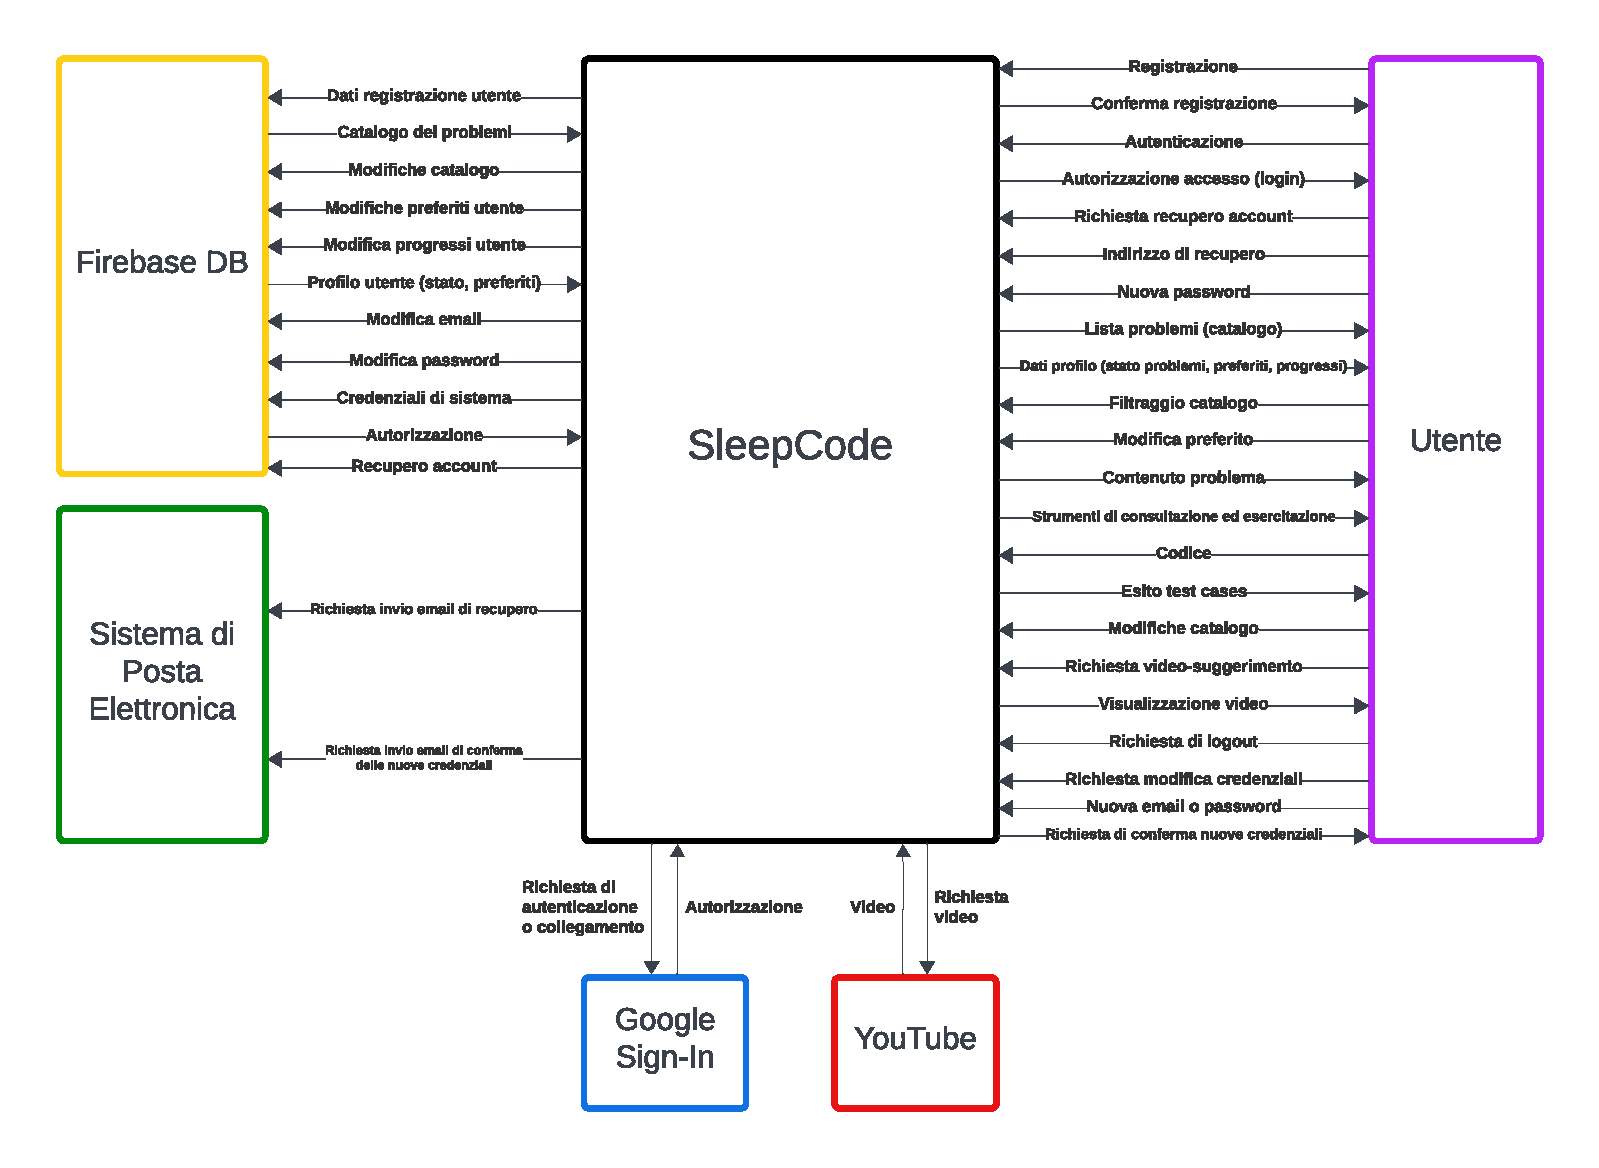
\includegraphics[scale=0.7]{materiale/contextdiagram.pdf}
\caption{Context Diagram della piattaforma Sleep Code}
\label{contextdiagram}
\end{figure}

\subsubsection*{Utente}
L'utente può richiedere di effettuare la registrazione alla piattaforma,
scegliendo di inviare i dati necessari per creare un
account di sistema (\textbf{RF 1}) o di collegare il proprio account Google (\textbf{RF 3}). Il sistema
provvede a inviare la conferma dell'operazione di registrazione.
L'utente registrato può inviare i dati necessari al login (\textbf{RF 2}) sulla piattaforma,
inserendo quindi le credenziali di sistema oppure richiedendo l'autenticazione
con Google. Il sistema risponde con l'autorizzazione all'accesso.
In caso di richiesta di recupero dell'account (\textbf{RF 4}) da parte di un utente
registrato, il sistema riceve l'indirizzo email di recupero. Dall'email
l'utente può collegarsi alla pagina di recupero, nella quale inserire la
nuova password dell'account.

L'utente riceve il catalogo contenente la lista di problemi disponibili,
con i relativi dati descrittivi (\textbf{RF 5}). Da qui, l'utente può
richiedere il suggerimento, con la conseguente visualizzazione da parte del
sistema. L'utente, selezionando uno dei problemi del catalogo, accede
all'area di esercitazione per consultare il contenuto del problema (\textbf{RF 6})
ed utilizzare gli strumenti di esercitazione (\textbf{RF 7}), con i quali
è possibile inoltrare al sistema il codice scritto e ottenere l'esito della
sua valutazione (\textbf{RF 8}). L'utente può inoltre manipolare il cronometro,
del quale il sistema mostra all'utente il tempo registrato (\textbf{RF 9}).

L'utente autenticato riceve informazioni sui preferiti, lo stato dei problemi
e sui progressi (\textbf{RF 10}, \textbf{RF 12.2}), fornisce la nuova password
per il proprio account (\textbf{RF 13}), la richiesta di logout (\textbf{RF 14})
e la richiesta di eliminazione dell'account (\textbf{RF 15}).
L'utente amministratore fornisce eventuali modifiche apportate al catalogo
(\textbf{RF 16}, \textbf{RF 17}, \textbf{RF 18}).

Per non appesantire il diagramma, sono stati omessi alcuni flussi di informazioni
di feedback ed esito da parte del sistema verso l'utente, che si ripetono in molti
scenari: \textit{Modifica password} (il sistema notifica la conformità della
nuova password inserita), \textit{Modifiche catalogo} (il sistema avvisa l'utente
circa eventuali modifiche non valide, come specificato dalle clausole
\texttt{[exception]} degli UC \textit{Aggiungere un problema} e \textit{Modificare
problemi}, Sezione \ref{consultazione}), \textit{Indirizzo di recupero} e
\textit{Nuova password} nell'ambito del recupero della password dell'account
(come specificato dalle eccezioni presenti nello UC \textit{Recuperare la
password}, Sezione \ref{accessoeautenticazione})

\subsubsection*{Firebase}
Firebase provvede alla memorizzazione del catalogo dei problemi, fornendoli
al sistema ai fini della loro visualizzazione, e dei dati associati agli utenti
registrati ed eventualmente autenticati (credenziali interne, preferiti,
progressi). Il sistema fornisce al database le informazioni ottenute in sede
di registrazione, consentendo agli utenti registrati mediante credenziali
interne o Google Sign-In di memorizzare un nuovo account (\textbf{RF 1},
\textbf{RF 3}); vengono inoltre fornite le credenziali specificate
dall'utente durante il login. Infine, l'esito della registrazione e del
login viene rappresentato dall'\textit{Autorizzazione}.

Questo attore esterno riceve anche le modifiche apportate
ai problemi (\textbf{RF 16}, \textbf{RF 17}, \textbf{RF 18}), ai dati
dell'account di un dato utente, quali preferiti, progressi, password e
accoglie richieste di eliminazione dell'account (\textbf{RF 10}, \textbf{RF 12},
\textbf{RF 13}, \textbf{RF 15}). In particolare, il sistema segnala al database
l'aggiornamento dello stato di un problema in relazione all'utente autenticato
che lo ha risolto, indicato da \textit{Aggiornamento progressi}
(\textbf{RF 12.1}).

\subsubsection*{Google Sign-In}
Google Sign-In fornisce l'autorizzazione per eventuali richieste di
registrazione e autenticazione mediante account Google (\textbf{RF 3}).

\subsubsection*{YouTube}
I video che l'utente intende visualizzare vengono richiesti a YouTube da
parte del sistema, per poi visualizzarli (\textbf{RF 5.1}).

\subsubsection*{Servizio di posta elettronica}
La piattaforma fornisce al sistema di posta elettronica i dati necessari
per notificare e guidare l'utente che intende effettuare l'operazione di
recupero dell'account (\textbf{RF 4}), quindi l'indirizzo di recupero e
il contenuto del messaggio che include il link di recupero.



\newpage
% diagramma componenti -> si intende componenti INTERNI AL SISTEMA:

% vantaggi componenti: se cambia uno degli attori (in particolare software)
% basta cambiare il rispettivo compnente con il quale si interfaccia

% il sistema non sarà un programma monolitico che si occupa di tutto con un unico codice
% provo a dividere il mio sistema in componenti e ragiono su come le informazioni vengono passate tra i componenti

\section{Analisi dei componenti}

Nella presente sezione viene introdotta l'architettura interna del sistema
rilevandone i componenti, definiti nei loro compiti sulla base dei requisiti
analizzati nelle sezioni e nei documenti precedenti. L'architettura viene
qui mostrata attraverso un Diagramma dei Componenti (Figura \ref{compdiagram}), che evidenzia
l'interconnessione tra i componenti interni, le interfacce presenti tra di
essi e quelle esposte agli attori esterni. Segue una descrizione testuale
e più dettagliata di ogni componente.

\subsection{Diagramma dei componenti}
\begin{figure}[H]
\centering
\hspace*{-3cm}
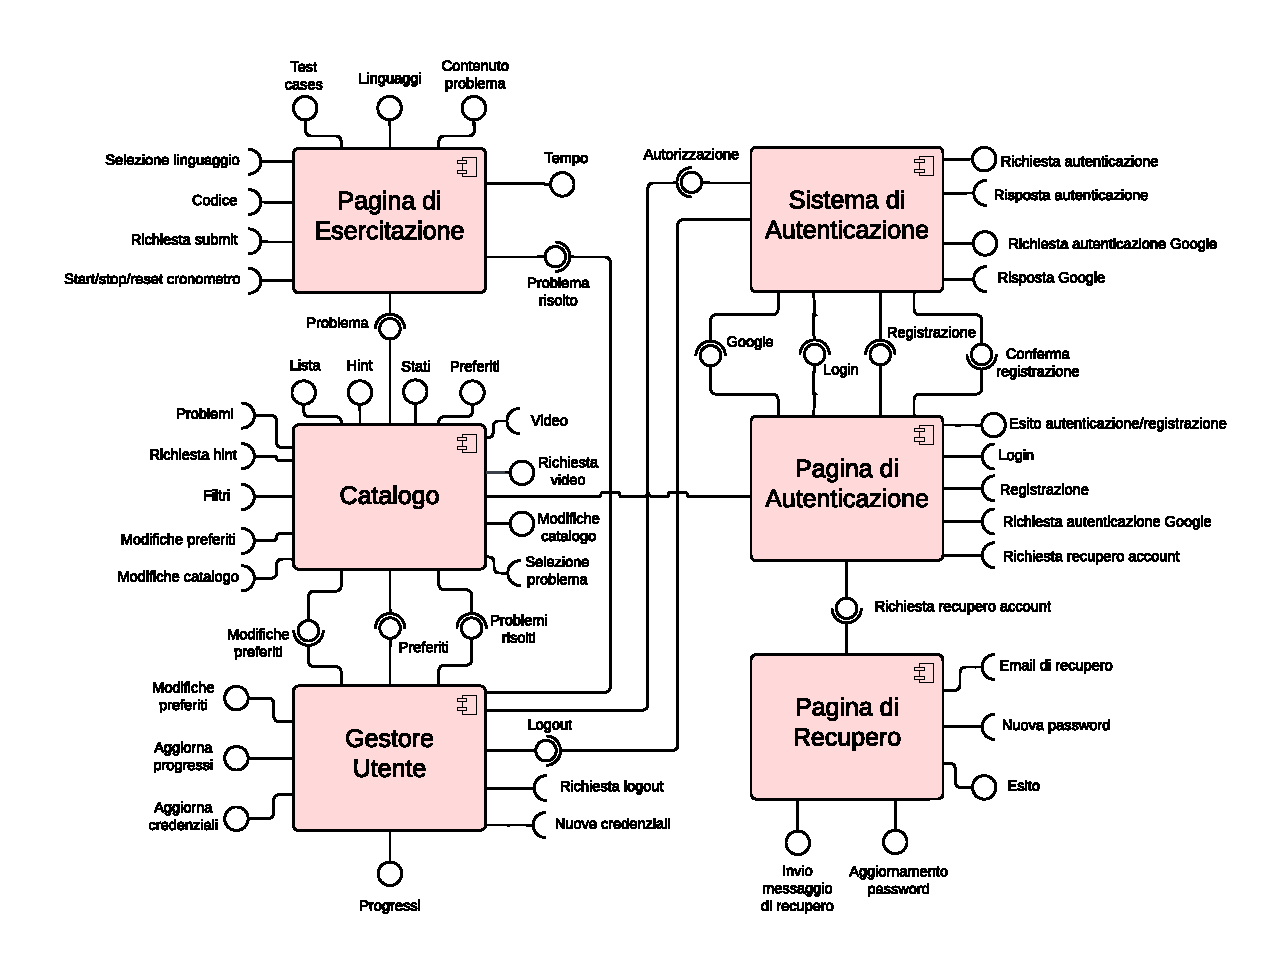
\includegraphics[scale = 0.86]{materiale/componentdiagram.pdf}
\caption{Diagramma dei Componenti del sistema Sleep Code}
\label{compdiagram}
\end{figure}

\newpage
\subsection{Definizione e descrizione dei componenti}
In questa sezione sono descritti i componenti e le interfacce presenti
all'interno del Diagramma dei Componenti, raffigurato in Figura \ref{compdiagram}.
Per ogni componente, viene fornita una breve descrizione che riassume gli
scopi e i principali compiti del componente in esame, elencando poi
le rispettive interfacce, a loro volta suddivise tra \textit{interfacce
richieste} e \textit{interfacce fornite}.

\begin{center}
    \rule{5cm}{1pt}
\end{center}

\subsubsection{Pagina di Autenticazione}

\begin{description}
    \item[Descrizione:] la Pagina di Autenticazione ha il compito
    di interagire esternamente con l'utente al fine di guidarlo nelle
    procedure di accesso alla piattaforma. Questo componente si occupa della
    raccolta dei dati utili ad effettuare la registrazione e il
    login. In più, esso raccoglie le richieste di recupero dell'account
    (la procedura effettiva è presa in carico dal componente
    \textit{Pagina di Recupero}).

    \item[Interfacce richieste:]
    \begin{itemize}
        \item[]

        \item \underline{Login:} questa interfaccia rappresenta
        il canale attraverso il quale l'utente immette le credenziali
        necessarie per richiedere di effettuare il login, ovvero
        \textit{email} e \textit{password}.

        \item \underline{Registrazione:} analogamente all'interfaccia
        di login, questa interfaccia include le credenziali utili alla
        creazione di un nuovo account (\textit{username, email, password}).

        \item \underline{Richiesta autenticazione Google:} la Pagina di
        Autenticazione accoglie eventuali richieste di autenticazione e
        registrazione mediante i servizi Google.

        \item \underline{Richiesta recupero account:} tramite il componente,
        l'utente richiede il recupero dell'account in caso di password
        dimenticata.

        \item \underline{Conferma registrazione:} la Pagina di Autenticazione
        riceve la conferma di registrazione (si veda \textit{Sistema di
        Autenticazione}), in modo da avvisare l'utente riguardo l'esito
        dell'operazione.

        \item \underline{Autorizzazione:} l'autorizzazione, prodotta dal
        componente \textit{Sistema di Autenticazione}, consente alla
        Pagina di Autenticazione di valutare l'esito dell'operazione di
        login, consentendo poi di avvisare l'utente.
    \end{itemize}

    \item[Interfacce fornite:]
    \begin{itemize}
        \item[]

        \item \underline{Esito autenticazione o registrazione:} sulla
        base delle informazioni ricevute per mezzo delle interfacce
        \textit{Autorizzazione} e \textit{Conferma registrazione},
        la Pagina di Autenticazione può avvisare l'utente circa
        l'esito delle operazioni, rispettivamente, di login e
        registrazione.

        \item \underline{Registrazione:} il componente inoltra la
        richiesta di registrazione, con credenziali annesse, verso
        il componente di competenza (\textit{Sistema di Autenticazione}).

        \item \underline{Login:} la Pagina di Autenticazione inoltra
        la richiesta di login, con credenziali annesse, verso il
        componente \textit{Sistema di Autenticazione}.

        \item \underline{Google:} il componente specifica eventuali
        richieste di autenticazione (o registrazione) con Google
        esponendo questa interfaccia.

        \item \underline{Richiesta recupero account:} le richieste di
        recupero vengono inoltrate al componente predisposto a questa
        operazione (\textit{Pagina di Recupero}).
    \end{itemize}
\end{description}


\begin{center}
    \rule{5cm}{1pt}
\end{center}

\subsubsection{Sistema di Autenticazione}
\begin{description}
    \item[Descrizione:] il Sistema di Autenticazione si occupa della
    gestione delle operazioni di login, occupandosi in particolare
    dell'autorizzazione dell'utente, determinandone il livello di
    accesso e di conseguenza la possibilità di usufruire di funzionalità
    fornite da alcuni componenti; inoltre, questo componente gestisce
    le operazioni di registrazione, dialogando esternamente con il
    servizio di database e Google.

    \item[Interfacce richieste:]
    \begin{itemize}
        \item[]

        \item \underline{Registrazione:} dalla Pagina di Autenticazione,
        questo componente riceve le credenziali allegate alla richiesta
        di registrazione.

        \item \underline{Login:} dalla Pagina di Autenticazione, il
        componente riceve le credenziali allegate alla richiesta di
        login.
        
        \item \underline{Logout:} dal Gestore Profilo, il componente
        riceve la richiesta di logout, permettendo di modificare di
        conseguenza il livello di accesso dell'utente.

        \item \underline{Google:} con la richiesta di questa interfaccia,
        il Sistema di Autenticazione viene a conoscenza di richieste di
        autenticazione con Google, in modo da effettuare la registrazione
        o il login interagendo appunto con Google.

        \item \underline{Risposta autenticazione:} questa interfaccia
        rappresenta l'esito, ricevuto tramite l'interazione con
        l'attore esterno \textit{Firebase}, sia dell'operazione di
        login che di quella di registrazione. Nel primo caso l'esito
        dipende dall'esistenza dell'account specificato tramite le
        credenziali ricevute dalla Pagina di Autenticazione e alla
        corrispondenza della tupla email-password, mentre
        nel secondo la risposta dipende dall'esistenza o meno di
        un account registrato con la stessa email specificata nella
        richiesta di registrazione.

        \item \underline{Risposta Google:} questa interfaccia rappresenta
        la controparte di quella precedente, ma essa permette al componente
        di comunicare con il servizio Google, sia per ricevere l'esito
        della registrazione che per quello del login.
    \end{itemize}

    \item[Interfacce fornite:]
    \begin{itemize}
        \item[]

        \item \underline{Richiesta autenticazione:} la richiesta di
        autenticazione viene rivolta dal Sistema di Autenticazione
        al servizio di database. Questa interfaccia permette di effettuare
        la validazione delle credenziali fornite nella richiesta di
        login.

        \item \underline{Richiesta autenticazione Google:} questa
        interfaccia è molto simile alla precedente, ma è predisposta
        all'invio della richiesta di login verso il servizio Google.

        \item \underline{Conferma registrazione:} il componente avvisa
        al componente Pagina di Autenticazione l'esito della
        registrazione mediante questo canale di conferma.

        \item \underline{Autorizzazione:} il componente comunica
        l'esito del login agli altri componenti del sistema, in modo
        tale da adattare la disponibilità delle funzionalità del sistema
        interno allo specifico livello di accesso dell'utente.
        Le informazioni erogate da questa interfaccia sono inoltre
        influenzate da eventuali richieste di logout da parte dell'utente.
    \end{itemize}
\end{description}

\begin{center}
    \rule{5cm}{1pt}
\end{center}

\subsubsection{Pagina di Recupero}
\begin{description}
    \item[Descrizione:] il componente, avvalendosi del servizio di posta
    elettronica, si occupa dell'operazione
    di recupero dell'account, offrendo assistenza a eventuali utenti,
    registrati con sistema di credenziali interno, che hanno dimenticato
    la propria password.

    \item[Interfacce richieste:]
    \begin{itemize}
        \item[]

        \item \underline{Richiesta recupero account:} il componente
        può attivare la procedura di recupero ricevendo la richiesta
        da parte della Pagina di Autenticazione.

        \item \underline{Email di recupero:} l'utente fornisce l'email
        associata all'account che si intende recuperare.

        %\item \underline{Nuova password:} dall'utente, il componente
        %ottiene la nuova password.
    \end{itemize}

    \item[Interfacce fornite:]
    \begin{itemize}
        \item[]

        \item \underline{Invio messaggio di recupero:} questa interfaccia
        rappresenta l'interazione del componente verso
        il servizio esterno di posta elettronica. Da qui, il
        componente richiede l'invio del messaggio di recupero,
        specificando inoltre l'email fornita dall'utente e il
        contenuto del messaggio.

        \item \underline{Esito:} l'esito dell'operazione viene
        fornito all'utente. Da qui, il componente può comunicare
        anche eventuali errori incontrati durante il recupero,
        come specificato nella descrizione dello use case
        \textit{Recuperare la password}, nella sezione relativa
        alla specifica dei requisiti funzionali.

        \item \underline{Aggiornamento password:} la Pagina di
        Recupero indica al database che la password dell'account
        deve essere modificata. L'interfaccia fornisce dunque
        la nuova password, allegata ad una richiesta di modifica
        delle credenziali presso l'account con email precedentemente
        specificata dall'utente.
    \end{itemize}
\end{description}

\begin{center}
    \rule{5cm}{1pt}
\end{center}

\subsubsection{Gestore Profilo}
\begin{description}
    \item[Descrizione:] il Gestore Profilo raccoglie le funzionalità
    associate principalmente all'utente autenticato, dedicandosi appunto alla
    gestione del suo \textit{profilo}, inteso come l'insieme delle informazioni
    raccolte nell'account, nei progressi e nei preferiti. In generale, questo
    componente deriva dalla scelta architetturale di gestire la disponibilità
    delle funzionalità fruibili dall'utente sulla base dei livelli di accesso
    anonimo e autenticato, definiti nel documento D1.

    \item[Interfacce richieste:]
    \begin{itemize}
        \item[]

        \item \underline{Autorizzazione:} il Gestore Profilo richiede l'autorizzazione
        prodotta dal Sistema di Autenticazione, in modo da rendere disponibili o
        meno le funzionalità accessibili a livello autenticato.

        \item \underline{Richiesta logout:} da qui l'utente può effettuare il logout.

        \item \underline{Modifiche preferiti:} questa interfaccia riceve le
        modifiche apportate ai preferiti dell'utente durante la navigazione
        nel catalogo, consentendo di aggiungere o rimuovere preferiti dal
        profilo.

        \item \underline{Nuova password:} attraverso questa interfaccia,
        l'utente può aggiornare la password del proprio account.

        \item \underline{Problema risolto:} da questa interfaccia, il Gestore
        Utente viene avvisato del fatto che l'utente ha risolto un problema.
        Sulla base dell'autorizzazione, che determina la distinzione tra
        utenti anonimi e autenticati, il componente può dunque valutare se
        sia necessario aggiornare i progressi dell'utente eventualmente autenticato.
    \end{itemize}

    \item[Interfacce fornite:]
    \begin{itemize}
        \item[]

        \item \underline{Preferiti:} il componente comunica al Catalogo la
        lista di problemi preferiti dell'utente autenticato, in modo da
        evidenziarli durante la navigazione.

        \item \underline{Modifiche preferiti:} le modifiche dei preferiti,
        apportate dall'utente, vengono memorizzate nel database.

        \item \underline{Progressi:} il componente mostra i progressi dell'utente,
        come descritto in \textbf{RF 12.2}.

        \item \underline{Aggiorna progressi:} questa interfaccia comunica al
        database di aggiornare i progressi dell'utente autenticato, nel caso
        in cui egli abbia risolto un problema.

        \item \underline{Problemi risolti:} il componente comunica al Catalogo
        quali sono i problemi risolti dall'utente autentiato, in modo da
        evidenziarli durante la navigazione.

        \item \underline{Aggiorna credenziali:} il componente interagisce con
        il database per aggiornare le credenziali dell'account, sulla base delle
        modifiche richieste dall'utente.
        
        \item \underline{Logout:} questa interfaccia propaga al
        Sistema di Autenticazione la richiesta di logout dell'utente autenticato.
        Questa interfaccia evidenzia come l'architettura stessa preveda che,
        dopo il logout, sia necessario eseguire il login passando ai componenti
        di competenza, ovvero la Pagina di Autenticazione e il Sistema di Autenticazione.
    \end{itemize}
\end{description}

\begin{center}
    \rule{5cm}{1pt}
\end{center}

\subsubsection{Catalogo}
\begin{description}
    \item[Descrizione:] questo componente consente ad un qualsiasi utente
    (anonimo, autenticato e amministratore) di consultare la lista di problemi
    disponibili sulla piattaforma, oltre a permettere di selezionare un singolo
    problema per aprirlo e iniziare a risolverlo, passando quindi alla \textit{Pagina di
    Esercitazione}.
    Il Catalogo facilita la navigazione visualizzando i dati descrittivi di ogni
    problema (nome, categoria, difficoltà), permettendo anche di eseguire ricerche
    filtrate per nome o altri campi; consente di visualizzare i suggerimenti;
    mostra lo stato di ogni problema e i
    preferiti alla vista dell'utente autenticato (e amministratore); permette
    agli utenti amministratori di gestire la lista dei problemi, aggiungendone di
    nuovi, modificandoli o eliminandoli.

    \item[Interfacce richieste:]
    \begin{itemize}
        \item[]

        \item \underline{Problemi:} il Catalogo ottiene la lista dei problemi
        memorizzati dal database.

        \item \underline{Richiesta suggerimento:} questa interfaccia
        viene esposta all'utente che intende selezionare, e visualizzare,
        il video-suggerimento associato ad un problema del catalogo.

        \item \underline{Selezione problema:} il Catalogo rileva la
        selezione di un problema specificato dall'utetne, così da
        poter avviare un'esercitazione su quel problema (il componente
        \textit{Pagina di Esercitazione} si occupa dell'esercitazione).

        \item \underline{Autorizzazione:} ricevendo l'autorizzazione
        da parte del Sistema di Autenticazione, il Catalogo può adattare
        la modalità di visualizzazione della lista dei problemi sulla
        base del profilo (preferiti, progressi) dell'eventuale utente
        autenticato. Inoltre, questa interfaccia indica al Catalogo
        se l'utente ha il permesso di modificare la lista dei problemi,
        riconoscendo l'accesso di un utente amministratore.

        \item \underline{Preferiti:} da questa interfaccia il Catalogo
        ottiene informazioni sui problemi preferiti dell'utente
        eventualmente autenticato, potendo così visualizzarli sulla
        lista, nel campo dedicato.

        \item \underline{Modifiche preferiti:} il Catalogo riceve
        dall'utente richieste di modifica dei preferiti, quali
        l'aggiunta o la rimozione di problemi specifici selezionati
        dalla lista.

        \item \underline{Problemi risolti:} il Catalogo riceve la
        lista di problemi risolti contenuti nel profilo dell'utente
        autenticato, in modo da poter contrassegnare tali problemi
        nel campo \textit{stato} durante la consultazione del
        catalogo.

        \item \underline{Modifiche catalogo:} da questa interfaccia,
        il Catalogo riceve i dati necessari per aggiungere o modificare
        un problema selezionato dall'utente amministratore, come
        descritto nelle specifiche dei requisiti funzionali. Infine,
        sempre da questa interfaccia vengono accolte richieste di
        eliminazione di problemi da parte di utenti amministratori.
    \end{itemize}

    \item[Interfacce fornite:]
    \begin{itemize}
        \item[]

        \item \underline{Lista:} il Catalogo mette a disposizione
        dell'utente la lista di problemi disponibili sulla piattaforma,
        mostrandone quindi i dati descrittivi, incluso il suggerimento.

        \item \underline{Richiesta video:} questa interfaccia ha lo scopo
        di interagire con l'attore esterno YouTube per richiedere la
        riproduzione del video-suggerimento selezionato dall'utente
        nel catalogo.

        \item \underline{Problema:} una volta che l'utente sceglie quale
        problema egli intende risolvere, il Catalogo fornisce tutti i
        dati di quel problema al componente \textit{Pagina di Esercitazione}.

        \item \underline{Stati:} sulla base del profilo ottenuto
        dal componente \textit{Gestore Profilo}, il Catalogo rende
        visibile all'utente autenticato il campo \textit{stato},
        dove vengono contrassegnati i problemi risolti dall'utente
        autenticato.

        \item \underline{Preferiti:} come per lo stato, questa
        interfaccia si riferisce alla visualizzazione, verso l'utente
        autenticato, dei problemi preferiti, come sempre in un
        campo dedicato durante la visualizzazione della lista.

        \item \underline{Modifiche preferiti:} questa interfaccia
        si occupa di comunicare al Gestore Profilo le modifiche
        apportate ai preferiti, su richiesta dell'utente autenticato
        che naviga nel catalogo dei problemi.

        \item \underline{Modifiche catalogo:} questa interfaccia
        comunica al database le modifiche apportate al catalogo
        da parte dell'utente amministratore.
    \end{itemize}
\end{description}

\begin{center}
    \rule{5cm}{1pt}
\end{center}

\subsubsection{Pagina di Esercitazione}
\begin{description}
    \item[Descrizione:] il componente consente di consultare il contenuto del problema
    precedentemente selezionato nel catalogo. Inoltre, la Pagina di Esercitazione mette
    a disposizione gli strumenti utili alla risoluzione dell'esercizio, provvede alla
    gestione della sottoposizione del codice e avvisa l'utente circa la correttezza dell'algoritmo.
    Qualora il codice sia corretto, questo componente si occupa di aggiornare i progressi
    dell'utente (autenticato) che ha risolto il problema, insieme allo stato di quest'ultimo
    in relazione all'utente in esame. Nel complesso, la Pagina di Esercitazione
    gestisce gli strumenti che compongono l'area di esercitazione.

    \item[Interfacce richieste:]
    \begin{itemize}
        \item[]

        \item \underline{Problema:} per operare, la Pagina di Esercitazione
        deve ricevere il problema selezionato precedentemente dal Catalogo.

        \item \underline{Selezione linguaggio:} il componente riconosce dall'utente il
        linguaggio di programmazione scelto per scrivere il codice (i linguaggi disponibili
        sono mostrati mediante un'interfaccia descritta tra le \textit{interfacce fornite}).

        \item \underline{Codice:} il componente ricevei il codice scritto
        dall'utente, in modo da poterlo sottoporre ai test cases.

        \item \underline{Richiesta submit:} dall'utente, la Pagina di Esercitazione
        riceve la richiesta di sottoposizione del codice.

        \item \underline{Start/stop/reset cronometro:} il cronometro integrato
        può essere manipolato dall'utente mediante questa interfaccia.
    \end{itemize}

    \item[Interfacce fornite:]
    \begin{itemize}
        \item[]

        \item \underline{Contenuto problema:} il componente si occupa di mostrare
        all'utente il contenuto del problema scelto (si intendono i dati strutturali:
        titolo, testo, esempi).

        \item \underline{Linguaggi:} la Pagina di Esercitazione mostra quali
        linguaggi di programmazione sono disponibili e selezionabili dall'utente.

        \item \underline{Test cases:} il componente visualizza i test cases
        (input fornito e output restituito dall'algoritmo scritto), insieme ai
        loro esiti.

        \item \underline{Tempo:} il componente si occupa di mostrare il tempo
        registrato dal cronometro.

        \item \underline{Problema risolto:} nel caso in cui tutti i test cases
        fossero corretti, in seguito ad una sottoposizione, il componente comunica
        tale informazione ad altri componenti (si veda \textit{Gestore Profilo}) per
        mezzo di questa interfaccia.
    \end{itemize}
\end{description}

\end{document}